\documentclass[11pt, twocolumn]{article}

% Packages
\usepackage{graphicx}
\usepackage{hyperref}
\usepackage{geometry}
\usepackage{amsmath}

% Additional package to allow for a subtitle
\usepackage[english]{babel}
\usepackage{titlesec}

% Page settings
\geometry{a4paper, margin=.75in}
\graphicspath{ {./images/} }

% Custom title and subtitle commands

\title{\vspace{-8ex}
    Dost \\ \vspace*{1ex}
  \large  CSE211 - Data Structures Term Project \\ \vspace*{1ex} Ahmet Hakan Candar \\ \vspace{1ex} 20220702022 \\ \vspace{-6ex}}

\date{}

% Document
\begin{document}

\maketitle


% Introduction
\section{Introduction}
Dost is a social network analysis app built with C++ and GTK4. It consists of a graphical and terminal user interface.
The project aims to show relations, suggest new friends, and detect communities among people.

% Project Description
\section{Methodology}
The project consists of three subprojects \texttt{lib}, \texttt{tui}, and \texttt{gui}. This modular approach
makes it easier to share components between graphical and terminal interfaces, and reduces development time. 

The \texttt{lib} subproject is a static library which implements Graph and Person structures, including their methods. 
Detecting communities is made possible with the Girvan Newman algorithm, which itself depends on edge betweenness, BFS, 
and DFS algorithms.

The \texttt{tui} subproject provides a simple terminal user interface for the user.

The \texttt{gui} subproject provides a graphical user interface for the user. This
is a much better alternative than the terminal interface, and offers an easier and tidier user experience.

Compilation of this project is made with the CMake build tool. CMake was selected for cross platform compatibility, 
advanced configuration, and automation. It is a popular choice among many other C/C++ projects and it is a familiar tool 
for many developers.

I had not created a CMake project that consisted of multiple subprojects before. I was also relatively new to GTK, 
but this project made me a lot more confident and experienced on these technologies. 


% Technologies Used
\section{Implementation}
The development first began with \texttt{lib} and \texttt{tui} subprojects in parallel. Implementing friend suggestion,
graph display, degree centrality and clustering coefficient was relatively easy. Girvan Newman algorithm, on the other hand,
required detailed research and some trial and error until it got working.

CMake build process made this parallel development easy and painless. The modular approach ensured there was clear separation 
between library and UI logic. 

After finishing the library and terminal interface, I began working on the graphical user interface. I selected GTK4 and libadwaita
for a modern look. It is not the easiest UI toolkit to work with, and requires some expertise in C and build tools. However, cross
platform compatibility and user friendly UI widgets outweighed its difficulty for me as a developer.

% Results
\section{Results}
The Girvan Newman algorithm detected five different communities, which makes sense after analyzing the graph data. Friend suggestion,
degree centrality and clustering coefficient algorithms worked like I expected. The graphical user interface ran without issues.

Thanks to the cross platform nature of the project, It has been deployed to and tested on four different operating systems, 
namely \textit{Arch Linux}, \textit{Fedora 40}, \textit{Ubuntu 23.10}, and \textit{Windows 11}. All builds ran smoothly.


% Conclusion
\section{Conclusion}
Lorem ipsum dolor sit amet, consectetur adipiscing elit, sed do eiusmod tempor incididunt ut labore et dolore magna aliqua. Ut enim ad minim veniam, quis nostrud exercitation ullamco laboris nisi ut aliquip ex ea commodo consequat. Duis aute irure dolor in reprehenderit in voluptate velit esse cillum dolore eu fugiat nulla pariatur. Excepteur sint occaecat cupidatat non proident, sunt in culpa qui officia deserunt mollit anim id est laborum

\newpage

\begin{tabular}{cc}
    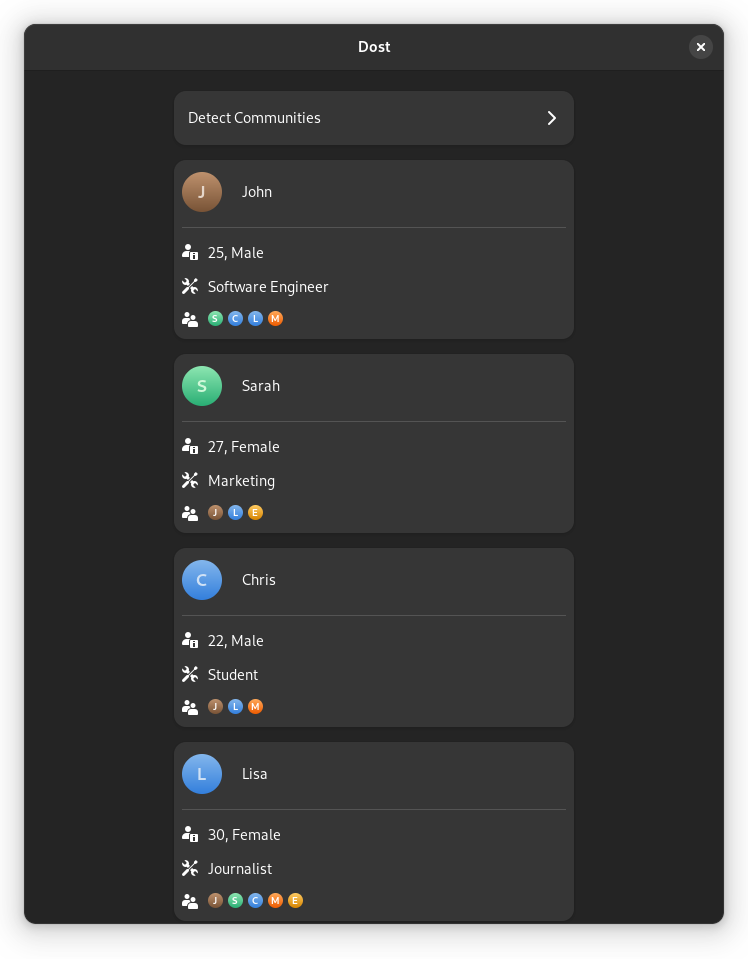
\includegraphics[width=.45\textwidth]{gui00} &
    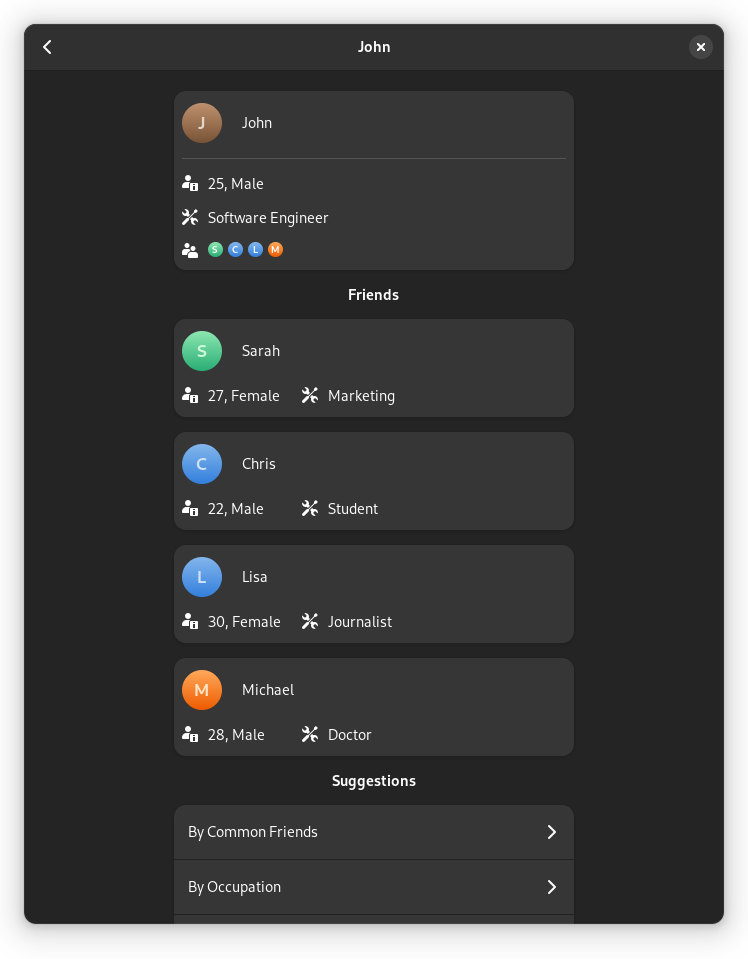
\includegraphics[width=.45\textwidth]{gui1}
     \\
     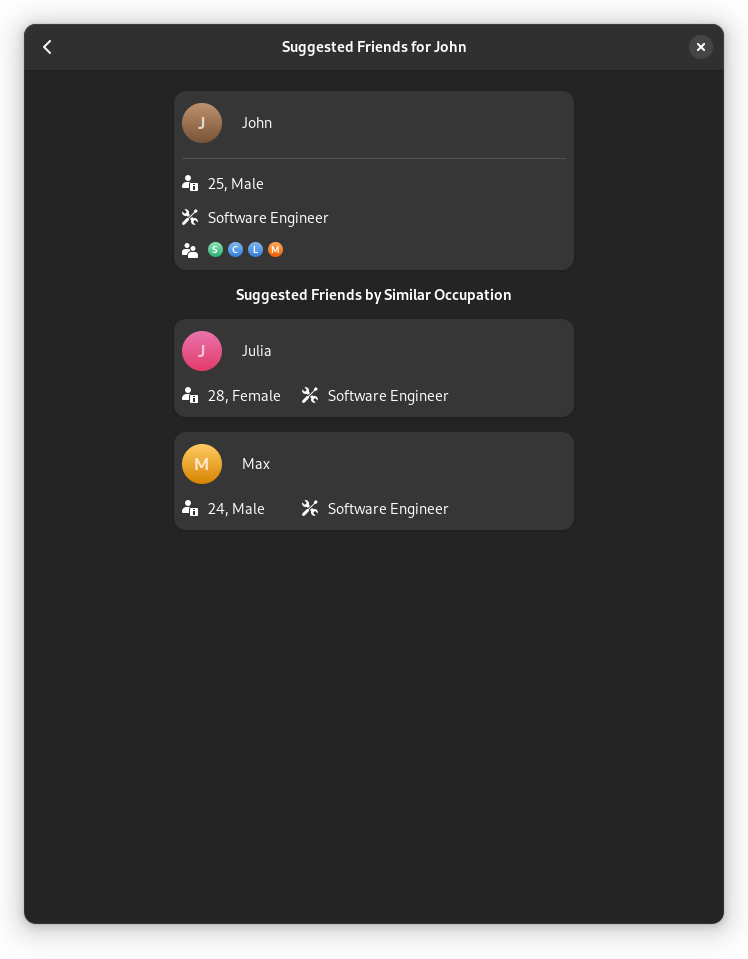
\includegraphics[width=.45\textwidth]{gui2} &
     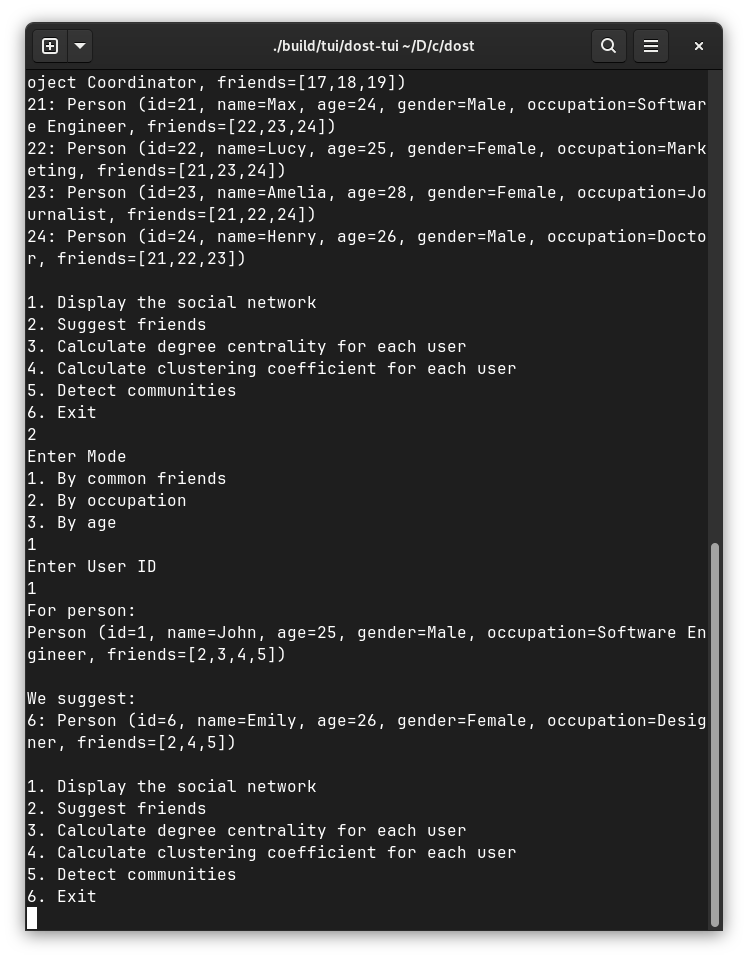
\includegraphics[width=.45\textwidth]{tui}
\end{tabular}


\end{document}
